
\chapter{海底热液系统} 
海底热液系统或者热液活动是洋壳内流体循环和水-岩反应等一系列复杂的相互作用的表现,热液流体在洋壳内循环并将能量和化学物质运输到地表(海底)。
水-岩化学反应导致了化学成分的运移,影响海洋和大气化学组成并且还会在海底形成具有经济效益的矿床\footnote{\href{ http://www.isa.org.jm/files/images/maps//Sulphides_Global.jpg} {国际海底管理局持续更新的海底多金属硫化物矿床分布图} } 。
海底热液活动也是地球的热引擎的重要组成部分,从岩石圈到地表的热传递以热传导、火山喷发和热液喷发的形式发生 \citep{LOWELL2014} 。
图 \ref{fig:ventFields_Global} 展示了全球海底热液区的分布\footnote{热液喷口位置来自Interridge数据库;
	板块边界和洋中脊坐标来自GPlate数据库;地形数据是对Etopo 1以10弧分的空间分辨率重采样得到。} ,
大约一半分布在洋中脊区域。
沿着火山洋中脊,当海水通过洋壳裂隙向下渗透过程中会发生热液循环。
海水首先被加热,在继续下渗的过程中与围岩发生反应,经历了化学改造,可达到的最高温度超过400 \ssd (图 \ref{fig:Hydrothermal_MOR} )。
在如此高温的条件下,流体密度会变的很小。
因此,流体在上浮力的作用下迅速上升,最后在海底以热液流体的形式喷出,与上覆海水混合。
海底热液循环在固体地球和海洋的能量和物质循环过程中扮演重要角色。

\begin{figure} [htbp] 
	\centering
	\includegraphics[width=\textwidth ]{vent_field_global} 
	\caption[海底热液活动全球分布]{海底热液活动全球分布} 
	\fnote{四种不同的形状表示不同的构造环境下的热液区:圆、三角形、正方形和旋转正方形分别表示洋中脊、火山弧、弧后扩张中心和板内火山。
		形状的不同颜色表示热液区的状态:灰色、橙色和红色分别表示非活动、低温和高温热液区。
		四种不同颜色的曲线表示不同扩张速率的洋中脊:如超慢速(Ultra-slow)扩张的西南印度洋脊 (SWIR: Southwest Indian Ridge) 和北冰洋的Gakkel洋脊;
		慢速(Slow)扩张的中大西洋脊 (MAR: Mid-Atlantic Ridge) 和中印度洋脊 (CIR: Central Indian Ridge);中速(Medium)扩张的东南印度洋脊 (SEIR: Southeast Indian Ridge);
		快速(Fast)扩张的东太平洋海隆 (EPR: East Pacific Rise) 和太平洋南极洲洋脊 (PAR: Pacific Antartic Ridge)。} 
	%	{热液区数据来源Interridge数据库:\url{http:www.interridge.org} } 
	\label{fig:ventFields_Global} 
\end{figure} 

\section{分布特征}  %参考海底热液地质学(曾志刚); German, 2006, Hydrothermal Processes

现代海底热液活动的分布范围广泛,主要分布在岩石圈板块离散和汇聚边界的区域。
在太平洋、大西洋、印度洋、北冰洋、南极洲、红海和地中海均有发现 (图 \ref{fig:ventFields_Global} )。
迄今为止,已发现的海底热液区(包括活动的、非活动的和热液异常点)多大~700处\footnote{\href{https://vents-data.interridge.org} {部分数据来自Interridge数据库} } ,
主要分布在太平洋 (约占63\%) ,其次是大西洋 (约占19\%) 、印度洋 (约占16\%) 、地中海 (约占3\%) 和北冰洋 (约占3\%) ,如图 \ref{fig:ventFields_Global} 和 \ref{fig:vent_stat_Oceans} 所示。
近30年来,据不完全统计,平均每年调查发现新的热液活动多大4处。特别是近十年,国际上投入洋中脊区域的调查研究时间平均 800d/a,平均有十段以上的洋中脊被调查。

\begin{figure} [htbp]
	\centering%
	\subcaptionbox{热液区在八大洋的分布\label{fig:vent_stat_Oceans} }  
	{\includegraphics[width=0.49\textwidth]{vent_stat_Oceans} } 
	\hspace{0.0\textwidth} 
	\subcaptionbox{构造环境及喷口状态\label{fig:vent_stat_Tectonic_T} }  
	{\includegraphics[width=0.4\textwidth]{vent_stat_Tectonic_T} } 
	\caption{热液区全球分布统计} 
	\fnote{Mediterranean:地中海;Indian:印度洋;N. Atlantic:北大西洋;S. Atlantic:南大西洋;N. Pacific:北太平洋;S. Pacific:南太平洋;\textcolor{red} {Southern} :。
		MOR:洋中脊;Arc:火山弧;Back arc:弧后扩张中心;Other:其他的构造环境,如板内火山、弧后盆地和裂谷深渊等。} 
	\label{fig:vent_stat_Ocean_Tectonic} 
\end{figure} 

从海底热液区所处的构造环境看,目前已发现的海底热液区有超过一半 (57\%) 分布在洋中脊,其次主要分布在火山弧 (21\%) 和 弧后盆地和扩张中心 (19\%) , 如图 \ref{fig:vent_stat_Tectonic_T} 所示。
随着对海底洋中脊区域的调查程度的不断提高,在南大西洋洋中脊、西南印度洋洋中脊、东南印度洋洋中脊、中印度洋洋脊、东太平洋海隆、极地海区以及西太平洋岛弧和狐猴扩张中心均有发现热液活动,
从而改变人们对于海底热液活动分布的构造环境方面的认识。
比如,早期发现的热液系统大部分是以玄武岩为基底,随着Rainbow热液区、Logatchev热液区、Lost City热液区、Saldanha热液区、Longqi热液区 \citep{tao2012first} 等在
超慢速扩张的西南印度洋洋脊和Gakkel洋脊上热液区的发现,
人们认识到沿着慢速和超慢速扩张、以岩浆集中供给为特征的洋脊,以超基性岩为基底的热液系统也普遍存在  \citep{schmidt2007geochemistry} 。


\begin{figure} [htbp]
	\centering%
	\subcaptionbox{柱状图 \label{fig:vent_stat_Spreading_Bar} } 
	{\includegraphics[width=0.49\textwidth]{vent_stat_Spreading_Bar} } 
	\hspace{0.0\textwidth} 
	\subcaptionbox{饼状图 \label{fig:vent_stat_Spreading_Pie} } 
	{\includegraphics[width=0.4\textwidth]{vent_stat_Spreading_Pie} } 
	\caption{洋中脊扩张速率及喷口状态} 
%	\fnote{} 
	\label{fig:vent_stat_spreading_T} 
\end{figure} 

海底热液循环系统主要存在于洋中脊,一个近乎连续的火山链,全长超过  $ ~6\times 10^4 $  km ( \ref{fig:ventFields_Global} )。
此洋中脊系统从北极盆地 (Arctic basin) 开始向南延伸,通过冰岛 (Iceland);然后继续向南延伸到中大西洋脊 (MAR),穿过Azores向南到达南大西洋;
在这里到达了Bouvet三联点 (50 $ ^{\circ}  S $ )。从此开始向西,一个主要的转换断层连接了将此三联点与Sandwich 和 Scotia 板块连接起来。
向东则是西南印度洋脊,向东北方向延伸知道Rodrigues三联点 ( $ ~ 25^{\circ}  $  S,  $ 70^{\circ}  $  E),洋中脊在此处分裂为两个分支。
其一是中印度洋脊 (CIR) ,向北延伸通过了西印度洋和亚丁湾 (Gulf of Aden) ,终止于初期海盆,也就是红海。
第二支是沿东南走向,从Rodrigues三联点形成东南印度洋脊和Pacific-Antarctic脊。这一分支穿过了整个南印度洋,
通过了Australasia (澳大拉西亚\footnote{一般指澳大利亚、新西兰和邻近南太平洋诸岛屿} )和南太平洋知道  $ ~ 120 ^{\circ}   $ W,洋中脊由此转向北延伸。
从此开始便是东太平洋海隆 (EPR) ,从  $ ~ 55 ^{\circ}   $ S 到  $ ~ 30^{\circ}   $ N,
在  $ ~ 30^{\circ}   $ N 与智利海隆 (Chile Rise) 相交,智利海隆连接了南智利海沟 (South Chile Trench)。
继续向北到赤道附近,Galapagos扩张中心与EPR相遇与另一个三联点。EPR最终终止于加利福尼亚海湾北部。
在这里,洋脊被知名的圣安德列斯断层 (San Andreas Fault) 分割为北西走向。

自首个热液喷口 (位于Galapagos扩张中心) 被发现以来,根据早期的观测数据得出了一个假说:沿着任何洋脊单位长度上热液喷口的发生率应该与其所在洋脊的扩张速率正相关,
因为扩张速率与洋脊所处位置的岩浆热通量 (岩浆供给量) 有本质联系 \citep{baker1996relationship} 。
也就是说,洋中脊扩张速率越大,其热液活动也越多,沿着超快速 (>140 mm/yr) 扩张洋脊 (EPR南部:  $ 17 - 19^{\circ}   $ S) 分布着最多的热液喷口 \citep{feely1996hydrothermal,ishibashi1997hydrothermal} 。
但是,近年来在全球洋中脊中慢速扩张脊上发现了广泛分布的热液喷口,
包括西南印度洋脊  \citep{tao2012first,german1998hydrothermal,bach2002discovery}   和格陵兰岛/北极盆地 \citep{edmonds2003discovery}  。
慢速-超慢速扩张洋脊上分布有大量热液区,这一事实无疑是对洋中脊热液系统的分布规律和其本质的传统认识的颠覆,为人们了解热液系统的本质提供了进一步线索。
如图 \ref{fig:vent_stat_spreading_T} 所示,目前发现的分布于超慢速扩张洋脊的热液区超过了超快速扩张洋脊的热液区数量,甚至是快速扩张洋脊的两倍之多。
此外,由于超慢速扩张洋脊地理位置偏远和探测条件的限制,目前对于超慢速扩张洋脊的调查研究程度依然不如快速和超快速洋脊的多 \cite{german2006hydrothermal} 。
从热液喷口活动状态和喷口温度统计关系来看,非活动热液喷口占大多数 (70\%) (图 \ref{fig:vent_stat_Spreading_Pie} );
而在活动热液喷口中,高温喷口总数多于低温喷口总数;慢速扩张洋脊上,高温热液喷口居多,而超慢速扩张洋脊上,低温热液喷口多于高温喷口 ( \ref{fig:vent_stat_Spreading_Bar} ) 。

\section{发现简史和意义}  %参考 LOWELL2014 (Hydrothermal Activity);海底热液地质学:曾志刚
对海底热液活动的直接探测始于1960年代,当时科学家们在沿着红海扩张脊轴 (慢速扩张) 的盆地采集的水样和沉积物中发现了金属颗粒  \citep{miller1964highest,miller1966hot,degens2013hot} 。
在1970年代,科学家们在中大西洋脊 (MAR) 发现了TAG 热液区  \citep{rona1975anomalous} ;在Galapagos扩张中心发现了温泉  \citep{corliss1979submarine} ,
对此处的喷口流体化学分析推测喷口流体来自于高温 (~ 350 \ssd) 的端元流体  \citep{edmond1979ridge}  。
直到1970年代末,在EPR 21  $ ^{\circ}  $  N 发现了第一个高温黑烟囱喷口,喷口流体温度为 350 \ssd \   \citep{spiess1980east} ;
自此,对海底热液活动的探测、采样和分析步入了一个新阶段。第一个高温热液喷口是在大西洋的TAG热液区被发现的  \cite{rona1986black} 。
 \cite{rona1980seafloor} 综述了一些列对海底热液活动的探测和发现有重大影响的研究工作,
针对海底热液系统的地质、地球物理、地球化学特征和探测方法等的研究被收录到了一些专辑 \citep{rona1983hydrothermal,wilcock2004subseafloor,german2004mid,lowell2008magma,rona2010diversity}  。
到目前为止,有超过700处的海底热液区被发现,
从超慢速到超快速扩张的洋中脊都存在高温热液喷口 (图 \ref{fig:vent_stat_Spreading_Bar} ),
而沿着洋中脊的热液喷口的分布是扩张速率的函数  \citep{baker2004global} ,
但是单个热液系统的热功率似乎与扩张速率无关  \citep{lowell2013characteristics} 。
具有代表性的几个热液区:2000年,日本科学家在CIR发现了Kairei热液区  \citep{gamo2001chemical}  ; 
2000年,美国科学家使用Alvin载人深潜器在大西洋中脊 30  $ ^{\circ}  $  N发现了Lost City热液区  \citep{kelley2001off} ,此低温热液区的发现对热液区的驱动热源又有了新的认识;
2001年,美国科学家在CIR距离Kairei热液区以北160 km处发现了Edmond热液区  \citep{von2001edmond} ;
1993-1994年,俄罗斯科学家在MAR发现了Logatchev热液区;
2007年,我国科学家在西南印度洋发现了首个活动的高温热液区-龙旂热液区  \citep{tao2012first}  。其他详细的探测发现历史参见  \cite{曾志刚2011海底热液地质学} 


这些热液系统的发现,导致了人们对地球上的生物-化学过程的认识彻底的改变了。
海底热液循环无疑对地球的全球地球化学物质循环有重要影响  \cite{edmond1979ridge} 。
此外,热液流体也是维持海底复杂的化能合成生物生态系统的能量来源  \cite{jannasch1995microbial} 。
海底热液系统附近的化能合成生物系统导致了人们对极端环境条件下的生命有了新认识,
并且激发了对地球和太阳系中其他行星上的生命起源的讨论和关注  \citep{baross1985submarine,nisbet2001habitat,mccollom1999methanogenesis,westall2013habitability} 。


\section{洋中脊热液系统}  %主要论述洋中脊热液系统的特征,不讨论分布
热液系统的驱动热源有多种,比如岩浆类 (Magmatic)、地幔上涌、化学反应放热(蛇纹石化:Lost City热液区)等。
洋中脊热液系统的驱动热源大多是岩浆房或者高温侵入岩(比如入侵的辉长岩),而岩浆类热源驱动的热液系统大多会形成高温热液喷口,
将这类热液系统称之为岩浆热液系统 (Magmatic Hydrothermal System)。
岩浆热液系统也存在于陆地上,但是其热液流体循环机制与洋中脊热液系统不同,如图 \ref{fig:HydrothermalSystemConcept} 所示的洋中脊和陆地热液系统概念模型。
从概念模型的角度出发,二者的区别在于边界条件、渗透率结构和流体性质。
比如,大陆浅层地壳的顶部边界条件是在一定的地形条件下的水体,因此流体是从地形高处向地形低处流动,如 \ref{fig:Hydrothermal_Continent} 所示。
相反,对于洋中脊热液系统,其顶部边界条件是静水压和海底处的海水温度,流体是从地形地处向地形高处流动,驱动力来源于被岩浆体加热之后的流体密度差异,如图 \ref{fig:Hydrothermal_MOR} 所示。
对于渗透率结构,陆地沉积岩比下覆结晶基底渗透率更高;而洋壳渗透率一般比上覆的细粒度海洋沉积物渗透率高。
对于流体性质,大陆上层地壳的循环流体一般为天然水,可能会溶解一些盐或者岩浆挥发物(比如CO $ _2 $ );而海底热液系统中的循环流体为盐度与海水相当的H $ _2 $ O-NaCl流体。



\begin{figure} [htbp]
	\centering%
	\subcaptionbox{陆地热液系统\label{fig:Hydrothermal_Continent} }  
	{\includegraphics[width=0.49\textwidth]{Hydrothermal_Continent} } 
	\hspace{0.0\textwidth} 
	\subcaptionbox{洋中脊热液系统\label{fig:Hydrothermal_MOR} } 
	{\includegraphics[width=0.49\textwidth]{Hydrothermal_Ocean} }  %HydrothermalSystem_MOR1
	\caption[热液系统模型图]{热液系统模型图(引自 \cite{ingebritsen2010numerical} )} 
%	\fnote{陆地} 
	\label{fig:HydrothermalSystemConcept} 
\end{figure} 

洋中脊附近的热液系统对地球的热平衡和全球化学、物质循环起到非常重要的作用。
热流研究一致表明洋中脊热液系统在地球总的热释放量中占比为20\%-25\%  \citep{sclater1980heat,stein1994constraints} ,而陆地热液系统只占 $ \sim $ 1\%  \citep{ingebritsen2010numerical} 。
如果没有洋中脊热液系统喷出的热液流体提供的溶质(矿物离子)和吸收某些溶质,
海洋则是以NaHCO $ _3 $ 为主导且pH值近乎10,而不是现在的以NaCl为主要成分且pH值接近8的海水 \citep{mackenzie1966chemical} 。
在洋中脊热液区附近发现的基于化学合成细菌的生态系统,为探索地球乃至其他行星的生命起源提供了线索 \citep{lutz1993ecology,baross1983growth} 。

\subsection{热液-热流}  %参考 LOWELL2014 (Hydrothermal Activity),German,Hydrothermal Process 的热通量部分
自首次在海底发现热液系统以来,
对其热流和对海洋化学的影响作用已有大量研究 \citep{edmond1979ridge,elderfield1996mid,stein1994constraints,schultz1997controls,german2006hydrothermal} 。
地球内部向外释放热量的总热通量为约为 42.2 TW,其中通过洋壳冷却的约为30.6 TW。
而通过洋壳释放的热通量中,以热液循环的形式占32.7 \% (10 TW),这些热液循环系统分布在从洋中脊到洋壳年龄为65 Ma的范围 \cite{stein1994constraints} 。
从图 \ref{fig:HeatFlux_ridge} 可以看出,在洋壳年龄在0-65 Ma范围内,实测热流值与岩石圈冷却模型得到的理论曲线有偏差,这部分偏差就是海底热液活动带来的热通量导致的结果。

\begin{figure} [htbp]
	\centering%
	\includegraphics[width=0.49\textwidth]{HeatFlux_ridge} 
	\caption[热流与岩石圈年龄的关系]{热流与岩石圈年龄的关系 \citep{LOWELL2014} 。} 
	\fnote{实线表示岩石圈冷却模型的理论曲线;
		点表示实测热流值,来自太平洋、大西洋和印度洋,并以2 Ma年为间隔进行平均;
		点线表示标准差;点划线表示对观测数据的拟合。} 
	\label{fig:HeatFlux_ridge} 
\end{figure} 

在洋中脊,岩浆类热源通过两种方式供热:(1)玄武质岩浆的结晶放热;(2)从洋壳冷却过程中汲取热量。
对于平均厚度为~ 6 km的洋壳,每年岩浆置换的质量约为  $ 6\times 10^{13}  kg/yr $ ,玄武质岩浆冷却到热液温度的过程中的最大放热约为  $ 2.8 \pm 0.3 TW $   \citep{elderfield1996mid,german2006hydrothermal} 。
假设这些热量全部以高温热液喷口的形式喷发,喷口温度为350\ssd 且海水压力\footnote{如无特别说明,本文中的{压力} 一词指的是{压强}  (Pressure),其国际单位为帕斯卡(Pa)} 为350 bar \footnote{压力常用单位:1 bar =  $ 10^5 $  Pa} ,则等效的物质体积通量为  $ 5-7 \times 10^{13}  kg/yr $ 。

\begin{figure} [htbp]
	\centering%
	\subcaptionbox{海水的等压比热容\label{fig:Cp_T_P} } 
	{\includegraphics[height=0.4\textwidth]{Cp_T_P} }  
	\hspace{0.05\textwidth} 
	\subcaptionbox{320 bar摩尔热容量与温度的关系\label{fig:Cp_Seawater_320bar} }  
	{\includegraphics[height=0.4\textwidth]{Cp_Seawater_320bar} } 
	\caption[海水的热容量与温度、压力的关系]{海水的热容量( $ c_p $ )与温度( $ T $ )和压力(P)的关系} 
	%	\fnote{陆地} 
	\label{fig:Cp_Seawater} 
\end{figure} 

但需要注意的是,海水(3.2\% NaCl溶液)的热容量( $ c_p $ )在热液的温压条件下对温度增加特别敏感(图 \ref{fig:Cp_Seawater} )。
比如当压力为320 bar、温度为400\ssd 附近时,温度的微小增加会使  $ c_p $ 增大一个数量级 (图 \ref{fig:Cp_Seawater_320bar} ),
从而导致运输同样多的热量,而水通量会减少  \citep{bischoff1985empirical,white1988heat,driesner2007system_part2} 。
当然了,并不是扩张脊轴部所有的热液热通量全部来自于高温热液流体。
 \cite{elderfield1996mid} 从全球尺度出发,考虑了一个均匀分布模型,
结果表明轴部\footnote{轴部 (axis):指的是洋中脊扩张脊轴;轴外或者离轴 (off-axis):指的是远离扩张脊轴的区域} 
集中喷发的高温热液流体 (热通量为  $ 0.2-0.4 \ TW $ ,物质体积通量为 $ 0.3-0.6 \times10^{13}  \ kg/yr $ ) 只占轴部总的热液通量的10\%。

在较老 (1-65 Ma) 的洋壳,热液循环受底部岩石圈地幔冷却过程中向上的传到热驱动。
这个过程中的热通量约为  $ 7 \pm 2 \ TW $   \cite{german2006hydrothermal} ,
远大于轴部和轴部附近的热通量总和,占地球上总的热液热通量的 75-80\%,占总的海洋热通量的 20\%以上以及地球总热通量的 15\%以上。
 \cite{mottl1994hydrothermal} 将与这部分热流有关的流体循环分为两部分:热的 (> 20 \ssd) 流体和冷的 (< 20 \ssd) 流体。
其中冷的流体携带 (或运输) 的热通量占离轴总热通量的88\%,对应的水通量为  $ 1-4 \times 10^{16}  \ kg/yr $   \citep{german2006hydrothermal} 。


\subsection{物理模型}  %code 参考 LOWELL2014 (Hydrothermal Activity)
热源和流体循环系统是热液活动的基本组成部分,热源从本质上决定了热液活动是高温 (> 150 \ssd) 还是低温的 \citep{LOWELL2014} 。
流体循环系统由注水区 (recharge zone) 和出水区 (discharge zone) 组成,海水通过前者进入洋壳被加热,从其周围环境中汲取能量和物质;
被加热的热液流体通过后者以热源或者热液喷口的形式出现在海底。
尽管流体在喷发之前可能经历了多次循环,此复杂的循环系统可以被简化为一个简单的单通道循环模型 (single-pass model)  \cite{LOWELL2014} ,见图 \ref{fig:SinglePassModel} 。

\begin{figure} [htbp]
	\centering%
	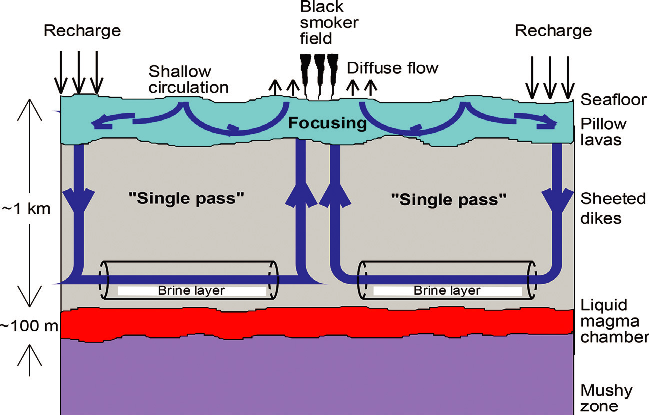
\includegraphics[width=0.49\textwidth]{SinglePassModel} 
	\caption[单通道模型示意图]{单通道模型 (Single-pass model) 示意图(引自 \cite{LOWELL2014} )} 
	\fnote{粗线表示的循环段代表了深部循环,海水渗透通过席状岩墙 (sheeted dikes) 直到岩浆房 (magma chamber) 顶部附近。
		汲取热量并经历水-岩化学反应,然后通过断层或者裂隙上升至海底,以黑烟囱的形式集中喷出。
		高温热液流体在上升的过程中,在浅部玄武质熔岩 (pillow lavas) 层与冷的海水混合,可能形成浅部低温循环并以弥散流 (diffuse flow) 的形式喷出。} 
	\label{fig:SinglePassModel} 
\end{figure} 

\subsubsection{热源}  %低温梯度-热传导;岩浆热源;化学反应放热
在地形高差作用下,存在于浅部 (~ 1-3 km) 地壳的低温热液系统,其驱动热源为地温梯度 ( $ H=\lambda dT/dz $ , $ \lambda $ 是热传导系数)。
比如在一个活动的火山区域,其低温梯度高达 100  $ ^{\circ} \text{C} /km $   \citep{LOWELL2014} 。
低温热液循环在洋壳中分布范围广泛,从洋中脊到岩石圈年龄小于65 Ma的范围内都存在 \citep{stein1994constraints} 。
此循环模式是海底地形、沉积厚度和类型、低温梯度和浅层洋壳 (~ 100 m) 的渗透率共同作用的结果  \citep{lowell1980topographically} 。
在所有海底热液活动中,低温热液活动造成的热损失超过了90\%  \citep{elderfield1996mid} 。
此循环对海洋地球化学的影响可以等效估计为:所有的海水在十万年内通过此循环全部进入地壳内 \citep{elderfield1996mid} ;
海洋中所有物质相当于海底热液循环喷发一千年的喷出物质质量总和 \citep{kadko1995magnitude} 。

高温热液活动与火山活动有关,浅部的岩浆侵入为热液循环提供热源。这类热源可以分为两部分,一部分来自于结晶放热;另一部分来自于岩体冷却。
在海底扩张中心,反射地震研究揭示了在1-3  $ km $ 范围内的浅部地壳存在岩浆房 \cite{carbotte2008variable,singh2006discovery} ,
在与扩张脊轴垂直的方向延伸1-2  $ km $ ,在沿着扩张脊轴的方向延展  $ ~ 10 km $  \citep{van2007seismic,jacobs2007axial} 。
由于岩浆房或者岩浆囊很薄 (~ 100 m) \citep{kent1990evidence,LOWELL2014}  ,
因此必须有深部岩浆对此岩浆房有足够快的补充速度才能维持实际观测到的热液输出功率量级 \citep{liu2009models} 。

橄榄岩的蛇纹石化 是一个可以产生热量的放热反应 \cite{macdonald1985rate} ,
改变演示化学性质并且由此形成了热液流体 \citep{janecky1986hydrothermal,wetzel2000distinguishing} 。
蛇纹石化不仅会形成独特的 (高碱度和非生物甲烷和氢气) 化学溶液 \citep{seyfried2004ultramafic} ,也会导致演示体积增加 (~ 40 \%) \citep{coleman1971petrologic,o1992solution} 。
蛇纹石化反应放热量取决于参与反应的岩石体积和蛇纹石化速率,其放热量足够驱动低温热液系统,热液流体温度从几摄氏度到几十摄氏度 \citep{lowell2002seafloor} 。
蛇纹石化发生的有利条件是海水能与大量的橄榄岩接触,比如低岩浆供给,形成薄的洋壳;构造拉张和体积膨胀形成断层或裂隙从而增加渗透率;上地幔岩石在海底出露。
这些条件大多会出现在慢速、超慢速扩张洋脊。
比如,Lost City热液区,洋壳与岩浆热源隔离  \citep{kelley2001off} 。这些蛇纹石化驱动的热液喷发流体温度高达75 \ssd,
并且沉淀出以碳酸钙和氢氧化镁烟囱为主要成分的高达60  $ m $  的烟囱。


\subsubsection{循环系统}  %渗透率;与裂隙和断层有关的渗透率;渗透率的时变特性
流体通过岩石运输热量,必然需要相互连通的流体流动通道和驱动力。
前者表示为渗透率 ( $ k $ ),而后者是由流体被加热后密度变化导致的上浮力,表现为流体的压力梯度。
热液流体在洋壳中的流动可视为流体在孔隙介质中的流动问题,其流动速度可以用达西定律 (Darcy's Law) 来表示:

\begin{equation} 
	\vec{v}  =- \frac{k} {\mu}  (\nabla P+\rho \vec{g} )
	\equcaption{达西定律} 
	\label{eq:DarcyLaw} 
\end{equation} 
其中  $ k $ 是介质的渗透率, $ \mu $ 为流体的动力学黏度; $ P $ 为压力; $ \rho $  为流体的密度; $ \vec{g}  $ 为重力加速度矢量。

岩石的渗透率 ( $ k $ ) 是影响热液循环的最为重要的物理参数,是裂隙和孔隙连通度的度量。
但是,此裂隙和孔隙连通度又受流体流动过程中的物理和化学作用的影响。
因此,对于一个特定的热液系统,其岩石的渗透率可能是时间和空间的复杂的函数。
此外,渗透率不仅是非均质各向异性的,还是与尺度有关的物理量,比如在较小的空间尺度,渗透率可能变化好几个数量级 \citep{LOWELL2014} 。

介质的孔隙度 ( $ \phi $ ) 表示的是岩石体积被流体占据的百分比。当这些孔隙彼此相连通时,可能形成供流体流动的通道。这种与孔隙度有关的渗透率成为初始渗透率。
孔隙度与渗透率之间的数学关系非常重要,因为孔隙度是一个与尺度无关的量,可以在实验室测量之;可以用电法和地震数据对孔隙度进行原位估计  \citep{LOWELL2014} 。
广泛使用的 $ k-\phi $ 关系是经典的Komeny-Carmen关系,可以表示为 \citep{civan2015reservoir} :
\begin{equation} 
	\left( \frac{k} {\phi} \right)^{1/2}  = \gamma \left( \frac{\phi} {1- \phi} \right)
	\equcaption{渗透率与孔隙度的关系} 
	\label{eq:K_phi_Relationship} 
\end{equation} 
其中 $ \gamma $ 是一个与颗粒大小和曲率有关的系数。

高温热液喷口大多是以火成岩或变质岩为基底的,这类岩石的孔隙度和初始渗透率都很低,对渗透率贡献较大的是裂隙。
当渗透率受断裂控制时,即使孔隙连通度很低的情况下依然可以形成较大的渗透率。
对热液活动区的演示渗透率的估计来自于钻孔测量、热液热通量的数学模型 \citep{lowell2013characteristics} 和
潮汐引起的海底压力扰动与喷口温度之间的相位差等 \citep{barreyre2016poroelastic,xu2017preliminary} 。
从ODP (Ocean Drilling Project) 和DSDP (Deep Sea Drilling Project) 
获得的钻孔数据得到洋壳渗透率范围从 席状岩墙的  $ 10^{-18}  \ m^2 $  
到枕状玄武岩的 $ 10^{-10}  \ m^2 $    \citep{fisher1998permeability,becker2013new} 。 
陆地热液系统的渗透率范围介于 $ 10^{-14}  - 10^{-17}  \ m^2 $ 之间  \citep{manning1999permeability} 。
对高温热液喷口的数学模型研究结果表明其渗透率范围在  $ 10^{-10}  - 10^{-14}  \ m^2 $ 之间 \citep{lowell2013characteristics,barreyre2016poroelastic,xu2017preliminary} 。
直接测量和模型研究都得到了大的渗透率值和变化范围,这也进一步说明了海底热液系统的渗透率是受裂隙或者断裂控制的。
尽管热液循环受裂隙和断层控制,但通常并不将其考虑为一些离散的裂隙去研究。
在数学模型中,通常将断裂的演示等效为孔隙介质并应用达西定律 (公式 \ref{eq:DarcyLaw} )  \citep{ingebritsen2010numerical,lewis2009numerical1,lewis2009numerical2,coumou2009phase,hasenclever2014hybrid} 。

渗透率随时间的变化可能是构造作用、岩浆作用、热学过程或者化学过程导致的。
当循环流体与到不同的温度和压力环境时,有可能沉淀 (precipitate) 或者溶解 (dissolve) 矿物。
比如在 ~100 bar的压力条件下,石英的溶解度 350 \ssd - 400 \ssd (取决于盐度) 达到了最大值  \citep{von1991quartz} 。
因此,如果热液温度超过400 \ssd ,则会沉淀出石英,从而堵塞裂隙和孔隙。
石英的沉淀会形成低渗透率的障碍,对热液流体的循环有重要的影响。
硬石膏的沉淀对注水区和出水区都有重要的影响 \citep{lowell2002anhydrite,steele2012role} ,因为硬石膏的溶解度随着温度的升高而降低。
海水在注水区被加热超过150 \ssd 时,会析出硬石膏;
当热的富含钙离子、缺少硫酸根离子的热液流体与冷的富含硫酸根离子、缺乏钙离子的海水混合时,同样会沉淀出硬石膏。
在海底以下混合,则会更有利于热液流体集中向黑烟囱喷发 \citep{lowell2003anhydrite,pascoe1996modelling} ;如果在海底混合,则会形成烟囱体 \citep{haymon1981hot} 。
当冷的流体流过热的岩石或者热的流体流过冷的岩石的时候会产生热弹性应力\footnote{Thermoelastic Stresses}  \citep{bodvarsson1976thermoelastic,lowell1990thermoelasticity,germanovich1992percolation} 。
前者会使岩石冷却收缩,导致渗透率增加;后者会使岩石受热膨胀,导致渗透率降低。渗透率与温度的关系可以表示为 \citep{germanovich2000stress} :
\begin{equation} 
	k=k_0 [1- \gamma (T-T0)]^3 + k_{res} 
	\equcaption{渗透率与温度的关系} 
	\label{eq:k_T} 
\end{equation} 
其中 $ k_0 $ 是主要裂隙网络的渗透率, $ k_{res}  $ 是剩余渗透率, $ \gamma $ 是表示热弹性效应强度的系数。
 \cite{lowell1993silica} 和 \cite{martin1997thermoelasticity} 研究表明热弹性效应比化学反应效应更快。当温度超过350-400 \ssd 时,岩石开始表现出韧性 (ductile),这种韧性会封堵断裂和裂隙。
因此,最初由于脆性破裂形成的渗透通道可能会逐渐闭合。

\subsection{热液活动的时变特性} 
在不同时间尺度上的变化是热液活动的基本特征 (图 \ref{fig:TimeScale_Hydrothermal} ),
这些变化与岩浆活动、构造活动或者气候变化有关。
这些过程发生的时间尺度从  $ ~ 10^6 - 10^7  $  年 (板块重构) 变化到  $ ~ 10^1 - 10^4  $ 年 (岩浆置换) 。
热液系统的时变性主要是地壳渗透率的变化和/或岩浆热源的衰减造成的,发生的时间尺度与为  $ ~ 1 - 10^2 $  年  \citep{lowell2002anhydrite,liu2009models}  。
随着地震、岩浆侵入 (如dikes) 或者火山喷发,洋中脊热液活动变化的时间尺度为几天到几个月  \cite{baker1987cataclysmic} 。
气候变化可能对沉淀模式有影响,因此会影响到流体注入 (recharge),其时间尺度为  $ 10 - 10^3 $  年;
冰期会对高纬度地区的热液系统有影响,由于海平面的下降,
从而海底压力减小,导致海底热液活动增强、物质通量增加、喷口温度上升 \citep{costa2017hydrothermal,lund2016enhanced,middleton2016hydrothermal} 。

\begin{figure} [htbp]
	\centering%
	\includegraphics[width=\textwidth]{TimeScale_Hydrothermal} 
	\caption[热液活动时间尺度]{与热液活动有关的事件和过程的时间尺度,依据 \cite{LOWELL2014} 。} 
%	\fnote{} 
	\label{fig:TimeScale_Hydrothermal} 
\end{figure} 

\subsection{喷口盐度变化}  %相分离
热液系统中沸腾的热液流体在海底以高温热液喷口的形式呈现,这类高温热液流体的温度一般介于 200 - 350 \ssd 。
对于纯水,其沸腾条件由其沸腾曲线 (温度的函数) 定义 (图 \ref{fig:PhaseDiagram_Seawater} )。
当温度低于沸腾点时,呈现为液相,反之呈现为现蒸汽相;沿着沸腾曲线,则两相共存,二者的体积分数取决于系统的焓的大小。
纯水的相图的最关键的特征就是其临界点\footnote{水的临界点 定义为:374 \ssd, 221 bar。超过临界点就会形成一种新的流体状态-超临界水。此状态下的液相和蒸汽相相互交融,已无区别。 }  (图 \ref{fig:PhaseDiagram_Seawater} )。
当温度和压力高于临界点时,以单相的超临界水的物质形态存在。

\begin{figure} [htbp]
	\centering%
	\includegraphics[width=0.5\textwidth]{SeawaterPhaseDiagram} 
	\caption[海水相图]{NaCl-H $ _2 $ O相图:温度( $ T $ )-压力( $ P $ )-盐度( $ X $ )关系图,修改自 \cite{driesner2007system_part1} 。} 
		\fnote{红色曲线和点表示纯水 (H $ _2 $ O) 的沸腾曲线和临界点;蓝色的曲线和曲面表示三相共存的界面;V: Vapor, L: Liquid, H: Halite。} 
	\label{fig:PhaseDiagram_Seawater} 
\end{figure} 
在海底黑烟囱处观测到的热液流体的盐度存在较大的变化,这是海底之下发生的热液流体发生相分离的表现 \citep{von1995evolution,von2003extraordinary} 。
海水从海底下渗进入洋壳,被岩浆热源加热上浮的过程中,
在一定的温度和压力条件(图 \ref{fig:PhaseDiagram_Seawater} ) 则会发生相分离,
形成密度高密度高盐度的卤水 (brine) 液相和低密度低盐度的蒸汽相 (图 \ref{fig:SinglePassModel} ) 。
多相热液系统可以分为以液相为主或以蒸汽相为主两类。

由于NaCl的存在,相分离过程在高于和低于海水临界点 (29.8 MPa, 407 \ssd, 3.2 wt \%) 两种情况下都有可能发生。
当相分离发生在压力低于临界点压力的情况时,海水将会沸腾,产生非常低盐度的蒸汽相和高盐度的卤水,形成以液相为主导的热液系统。
系统压力分布趋近于静水压,在地表出水区表现为沸腾的热泉,这类热液流体的pH一般呈中性-碱性且富含Cl。
相反,当温度-压力条件高于临界点时,分离出少量的卤水并凝结并向下流动,
剩余的大量的蒸汽相则会携带有较大的盐度 (取决于温度-压力条件)  \citep{coumou2009phase} ,形成以蒸汽相为主导的热液系统。
压力在蒸汽相主导的区域内近乎均匀分布且一般比静水压低 \citep{white1971vapor} ,


\section{慢速-超慢速扩张洋脊热液系统}  
%参考:Rona,2013专辑(Diversity of Hydrothermal Systems on Slow Spreading Ocean Ridges)
最近的研究表明,位于慢速和超慢速扩张洋中脊(全扩张速率小于30 mm/a)的热液系统与位于中速到快速扩张洋中脊的热液系统有极大的不同,
与其基底岩石圈的地质学特征的不同有关 \citep{rona2010diversity} 。
当第一个高温黑烟囱在EPR于1979年被发现时,科学家们一致认为只有中速到快速扩张的洋中脊有相对较高的岩浆供给才可以维持这样的热液活动,而在慢速-超慢速扩张的洋中脊应该不会出现高温热活动。
直到1985年,第一个高温热液喷口在慢速扩张的MAR上的TAG热液区被发现 \citep{rona1986black} ;
2002年在超慢速扩张的Gakkel洋脊上发现了高温黑烟囱 \citep{edmonds2003discovery} ;
2006年在超慢速扩张的西南印度洋发现了第一个高温热液喷口 \citep{tao2012first} 。
存在于超慢速扩张洋脊的热液系统与中速、快速扩张洋脊的热液系统之所以不同,原因在于岩浆供给速率、围岩 (基底岩石) 类型、
岩浆活动和构造拉张之间的相互作用之间的差异。

\subsection{热源类型}  
%参考 Lowell, 2020 (Hydrothermal circulation at slow spreading ridges: analysis of heat sources and heat transfer processes)
在快速和中速扩张洋脊,有越来越多的证据表明热液循环系统是靠近轴部岩浆房的 \citep{singh2006discovery,canales2006seismic} ,
地震成像研究对此岩浆房的空间展布和厚度 \citep{detrick1987multi,kent1990evidence,van2007seismic,jacobs2007axial} 以及底部部分熔融区的范围 \citep{dunn2000three} 已有较为准确的认识。
而在超慢速扩张洋脊,岩浆供给速率较小且呈现出间歇性特征,部分熔融区范围更小 \citep{sinton1992mid} 。
但是,热液活动倾向于在岩浆或者火山活动区附近形成。
一方面,反射地震研究表明岩浆房在Luck Strike \citep{singh2006discovery} 和Snake Pit \citep{calvert1995seismic} 热液区的深度分别为3 km和1.2 km。
甚至在超慢速扩张的Gakkel洋脊,热液活动似乎与新生火山活动有关 \citep{michael2003magmatic,baker2004hydrothermal} 。
另一方面, \cite{canales2007crustal} 利用地震数据并没有探测到TAG热液区之下的浅部至中部洋壳存在岩浆房。
有可能岩浆房存在于较深的地壳或者上地幔,只是目前还没有探测到;
但是,微震观测数据表明在TAG热液区以下 ~ 7 km范围内依然有天然地震存在,从而推测热液循环可能沿着拆离断层穿透到更深的地壳 \citep{sohn2007kinematics} 。
与TAG情况类似,龙旂高温热液区之下也没有探测到岩浆房 \citep{niu2015along,zhao2013three,li2015seismic} ,但是天然地震存在于更深的范围内\footnote{论文准备投稿 (Tao, et al., 2019)} 。
此外,在龙旗热液区 (位于28洋脊段) 附近的断桥区域 (位于27洋脊段) 海底以下9 km 范围内探测到了轴部岩浆房 \citep{jian2017evidence} ,但是此脊段上的断桥热液区已不再活动。
虽然岩浆热源对于慢速扩张洋脊上的热液系统很重要,但是化学反应 (比如蛇纹石化) 放热同样也有重要作用。
此外,用于驱动热液循环的热源有可能直接来自地幔、地壳和岩石圈冷却。

\subsubsection{地幔上涌} 
地幔直接传递的热通量大小可以用简化公式表示为 \citep{lowell2010hydrothermal} :
\begin{equation} 
	H_M \approx [\rho_r c_r (T_M - T_0) + \rho_r L]\mu_M \times 10^6 \ W/km^2
	\label{eq:HeatFlux_Mantle} 
\end{equation} 
其中 $ T_0 $ 表示地幔冷却的背景温度, $ L = 5 \times 10^5\ J/kg $ 表示结晶放热量,
 $ \rho_r = 3.3\times 10^3 \ kg/m^3, c_r = 10^3 \ J/kg/^{\circ} \text{C}  $ 和 $ T_M = 1300^{\circ} \text{C}  $ 分别表示
地幔岩石的密度、比热和温度, $ \mu_M = 0.01\ m/a $ 表示慢速扩张洋脊的地幔上涌的速度。
通过公式 \ref{eq:HeatFlux_Mantle} 可以算得到慢速扩张洋脊的地幔热通量为  $ H_M \approx 1.8 \ MW/km^2 $ ,
而慢速扩张洋脊上的热液系统的热功率为  $ 1062 - 10^3 \ MW $   \citep{lowell2010hydrothermal} 。
为了达到这样的热输出功率,热液系统须从 $ 10^2 - 10^3 \ km^2 $ 范围内汲取热量。
即使满足了热通量的需求,而最终的喷口温度也是不确定的。
假如地幔热源为一个高温的单相热液系统供热,则此热液系统需要一个非常理想化的渗透率分布。
因此,地幔热源直接驱动高温热液系统似乎不可能。

\subsubsection{洋壳和岩石圈冷却} 
最早的热液循环模型是用来解释观测到的传到热流与岩石圈冷却模型之间的负差现象 (图 \ref{fig:HeatFlux_ridge} ) 。
当第一个高温热液喷口被发现时 \citep{spiess1980east} 后,很多研究试图解释观测数据是从洋壳中汲取热量的结果。
但是很快人们意识到,在这种机制下,高温热液喷发不能维持很长时间 \citep{strens1982model,lowell1985hydrothermal} ,
从此引入了岩浆热源 \citep{cann1982black,lowell1985hydrothermal,lowell1991numerical} 。

%流体在裂隙中循环,从洋壳岩石中传热
\textbf{流体在裂隙中循环,从洋壳岩石中传热}   \citep{bodvarsson1972ocean,lowell1975circulation,strens1982model} 。
这个问题可以用一个简化的模型通过计算来说明:温度为  $ T_{f0}  $  的冷的流体进入一个裂隙 (长度、宽度和高度分别为  $ l,d $ 和  $ h $ ),
这个裂隙是独立的嵌入在初始温度为  $ T_{r0}  $ 的热的岩石中的,并且流体是从深部朝着海底以速度  $ u_f $ 向上流动的,
到达海底离开岩石时的温度为  $ T_f(h,t) $ ,这个正是我们需要求解的量,表示喷口流体的温度。
这是一个通过岩石进行热传导和通过流体流动进行热传递的综合问题,用数学语言表示为:

%\begin{equation} \label{bilevel} 
%	\left\{\begin{array} {l} 
%		\max\limits_{{\mbox{\footnotesize\boldmath  $ x $ } } }  F(x,y_1^*,y_2^*,\cdots,y_m^*)\\[0.2cm]
%		\mbox{subject to:} \\[0.1cm]
%		\qquad G(x)\le 0\\[0.1cm]
%		\qquad(y_1^*,y_2^*,\cdots,y_m^*)\mbox{ solves problems } (i=1,2,\cdots,m)\\[0.1cm]
%		\qquad\left\{
%		\begin{array} {l} 
%			\max\limits_{{\mbox{\footnotesize\boldmath  $ y_i $ } } } f_i(x,y_1,y_2,\cdots,y_m)\\[0.2cm]
%			\mbox{subject to:} \\[0.1cm]
%			\qquad g_i(x,y_1,y_2,\cdots,y_m)\le 0.
%		\end{array} \right.
%	\end{array} \right.
%\end{equation} 

\begin{equation} \label{eq:HeatTransferFractures} 
	\left\{\begin{array} {ll} 
		\frac{\partial {{T} _{r} } (x,t)} {\partial t} ={{K} _{r} } \frac{{{\partial } ^{2} } {{T} _{r} } (x,t)} {\partial {{x} ^{2} } }  & \text{\small{岩石热传导} }  \\ 
		{{\rho } _{f} } {{c} _{f} } d{{u} _{f} } \frac{\partial {{T} _{f} } (z,t)} {\partial z} ={{\left. -2{{\lambda } _{r} } \frac{\partial {{T} _{r} } (x,t)} {\partial x}  \right|} _{x=0} }  & \text{\small{本构方程: 岩石传导热=流体流动传热} }  \\
		{{T} _{r} } (x,0)={{T} _{r0} }  &\text{\small{初始条件} }  \\
		{{T} _{f} } (0,t)={{T} _{f0} }  &\text{\small{边界条件1: 底部流体温度=入水温度} }  \\
		{{T} _{f} } (z,t)={{T} _{r} } (0,t) &\text{\small{边界条件2: 两壁流体温度=岩石温度} } 
	\end{array} \right.
\end{equation} 
其中 $ K_r $ 和 $ \lambda_r $ 分别表示岩石的热扩散系数和热传导系数, $ \rho_f $ 和 $ c_f $ 分别表示流体的密度和比热。
以上方程的解可以表示为 \citep{bodvarsson1969temperature,lowell1976comments} ,
\begin{equation} 
	T_f(z,t)=T_{f0}  + (T_{r0}  - T_{f0} )\text{erf} \left[\frac{\lambda_r z} {2c_f q\sqrt{K_r t} } \right]
	\label{eq:Solution_HeatTransferFractures} 
\end{equation} 
其中erf表示误差函数\footnote{在数学中,误差函数又被称作高斯误差函数(S形状)。定义为一个积分:  $ \text{erf} (x) = \frac{2} {\sqrt{\pi} } \int_{0} ^{x} e^{-t^2} dt $ .  $ \text{erf} (\infty)=1 $ } , $ q=\rho_fc_fu_f d $ 表示裂隙单位长度上的物质通量。

令 $ z=h $ 表示海底,如果给定初始温度和流动速度等,根据 $ T_f(h,t) $ 就可以计算出喷口流体的温度随时间的演化。
比如假设 $ h=2000 \ m, T_{r0} =400^{\circ} \text{C} , T_{f0} =100^{\circ} \text{C}   $ 。
由公式 \ref{eq:Solution_HeatTransferFractures} 可知,喷口流体初始温度为400 \ssd,
随着时间的推移而温度降低。
为了了解热液系统的持续时间与通量之间的关系,假设喷口温度降低到 300 \ssd ,
则根据公式 \ref{eq:Solution_HeatTransferFractures} 可以计算得到误差函数的值为:
\begin{equation} 
	\text{erf} \left[\frac{\lambda_r h l} {c_f Q\sqrt{at} } \right] = \frac{T_f(ht) - T_{f0} } {T_{r0}  - T_{f0} }  = \frac{300-100} {400-100}  = 0.67
	\label{eq:erf_300} 
\end{equation} 
其中 $ Q=ql $ 表示总的物质流动速率,单位为 $ kg/s $ 。当误差函数erf的值介于[0,0.7]范围内时,可将其视为一个线性函数。
因此当喷口温度减小到低于310 \ssd 的情况下,误差函数的值随着 $ t^{-1/2}  $ 减小。
而对于一个给定的喷口温度,换言之,如果某热液喷口温度要保持在某个值,根据公式 \ref{eq:erf_300} 不难看出需要在 $ Q $ 和 $ t $ 之间权衡。
当热液活动生命期  $ t $ 越长,则流动速率 $ Q $ 必须要慢。
对于一个特定的热液系统,流动速率可以根据观测的热功率进行计算。
比如典型的热液系统 \citep{lowell2013characteristics} 具有350 \ssd 的喷口温度和 $ H_f \approx 10^9\ W $ 的功率,则物质流速率 $ Q $ 可以计算得到,
\begin{equation} 
	Q = \frac{H_f} {c_f \delta T}  \approx \frac{10^9} {6 \times 10^3 \times 350}  \approx 500 \ kg/s
	\label{eq:MassFlowRate_350} 
\end{equation} 
将此物质流速率带入公式 \ref{eq:erf_300} ,假设裂隙长度 $ l=1000 \ m $ ,热力学参数见附表 \ref{tab:append_Symbols_Values} ,我们可以计算出喷口温度从400 \ssd 降低到 300 \ssd 所需要的时间约为  $ 10^6\ s $ 。
这与  \cite{strens1982model}  和  \cite{lowell1985hydrothermal} 得出的结果一致,故黑烟囱热液循环不足以由其从单个裂隙或者断层区域围岩中汲取热量来维持。


%流体下渗迁移传热

%环型对流和岩石圈冷却

%\subsection{形成条件} 

\subsection{影响因素} 
% 参考: Lowell,2003(Anhydrite precipitation and the relationship between focused and diffuse flow in seafloor hydrothermal systems)
% Lowell, 2013 (Characteristics of magma‐driven hydrothermal systems at oceanic spreading centers)
% Matthew, Lowell, 2012 (The role of fluid phase immiscibility in quartz dissolution and precipitation in sub-seafloor hydrothermal systems)

\section{热液系统研究方法} 
% 参考:Coumou 2008,博士论文
目前对海底热液系统的研究方法有直接观测、间接观测和数值模拟三大类。
直接观测的难度大、费用高、观测数据稀疏,比如对喷口流体测温、采样,很难做到长周期大范围测量。
在过去几十年,利用载人和无人深潜器能够直接获取热液系统的一些观测数据 \citep{von2003extraordinary,charlou1996mineral} ,
对海底以下的热液对流单元\footnote{Convection Cell} 大小以及运输能量和物质的量级有了直接的认识。
到目前为止,在所有的扩张边界都找到了活动的热液喷口,水深变化范围从800 m到3600 m \citep{von2001edmond} 。
热液区的面积为  $ 10^3 - 10^5 \ m^2 $  \footnote{相当于几个到几十个足球场的面积} ,一般由几十个单独的黑烟囱组成 \citep{lowell1995seafloor} 。
高温热液喷口的温度最高可以接近 400 \ssd,但从来不会超过400 \ssd 。
几乎在所有的热液区都观测到了低温 (< 100 \ssd) 弥散流,这些弥散流一般分布在高温热液喷口附近和热液区的边缘 \citep{hannington1995physical} 。
对一些个别的热液区的研究表明,大部分 (> 90\%) 的对流热损耗是由弥散的低温的喷发造成的 \citep{lowell1995seafloor} 。
与黑烟囱相对应的还有一类温度介于 100 \ssd 至 300 \ssd 的喷口,称之为白烟囱,因为这类喷口会沉淀出白色颗粒物,如二氧化硅、硬石膏和重晶石 \citep{hannington1995physical} 。
目前所观测到的喷口流体的盐度都与海水的盐度存在差异 \citep{von2003extraordinary} ,盐度的这种高或者低异常只能用深部发生的相分离过程来解释 \citep{coumou2008numerical} 。
相分离过程是影响热液系统的物理和化学性质的关键过程,由于相分离对金属的溶解度有很大影响,所以对矿床的形成也有特殊影响。
金属会有限分馏溶解于流体 (液相或者蒸汽相) ,然后通过流体流动来实现其运输。

\subsection{地球物理观测} 
相对于直接观测数据,地球物理观测数据对海底之下的热液系统和与之相关的热通量的研究提供了重要的约束信息。
地震观测数据可以提供上地壳的结构,探测到轴部岩浆房或者熔融透镜体 \citep{dunn2000three} 。
然而,在慢速扩张洋脊,地震观测数据并没有反映出热液系统下方存在熔融体。
对海底热流的观测尤其重要,对全球洋中脊区域的热流估计并发现了实测数据与岩石圈冷却模型预测的热流曲线存在差异 \citep{stein1994constraints} 。
实际上正是这二者之间的差异,激发了人们对洋中脊热液活动的探测。
对一个稳定状态的热液喷口的输出功率最高估计,可以通过洋壳增生过程附加的能量来计算,结果为 $ 10 - 120 MW/km $ ,与扩张速率有关 \citep{coumou2008numerical} 。
但是对热液系统和洋脊段的热流观测却反映出更高的输出功率,可能是岩浆供给的周期性的而且是局部供给模式 \citep{baker1987cataclysmic,baker1996relationship,ramondenc2006first,germanovich2015measuring} 。
地球物理方法并不能直接得到热液对流单元的结构,但是一些方法却给出了非常有价值的结论。
磁异常数据可以反映出热液上流通道,因为在这个区域的岩石中的磁性物质被淋滤进入热液流体,导致在海底附近产生低的磁异常。
比如在Main Endeavour热液区,热液流体上升通道较窄、呈近乎数值的管状特征 \citep{tivey2002crustal} 。
微震数据可能会反映出注水区 (循环下渗通道),微震活动的纵向延伸范围被认为是反应出热液循环的最大深度范围。
最近有微震数据推测注水区可能直接到达岩浆透镜体上方,距离海底约  $ 2-4\ km $  \cite{tolstoy2008seismic} ,
 \cite{sohn2007kinematics} 基于微震数据推测TAG热液区的拆离断层为流体下渗提供通道,热液循环可能达到海底以下  $ 9\ km $ 之深。
热液循环单元结构的其他证据来自蛇绿岩 (ophiolite),从化石中可以推断出热液上升通道是近似管状结构 \citep{saccocia1995hydrothermal} 

\subsection{周期性观测} 
对热液喷口流体的长周期观测发现一些化学和热学性质在长时间 (几十年) 内保持不变,而一些其他性质则会在周 (week) 时间尺度内变化 \citep{von2003extraordinary,massoth1989submarine,von1990seafloor,von1997direct} 。
在一些区域观测到喷口流体温度随着地震的发生而变化 \citep{fornari1998time,johnson2000earthquake,pontbriand2014microearthquake} 。
对此有学者提出了几种机制解释温度扰动的现象:破裂前缘的传播和岩浆置换 \citep{wilcock2004physical,germanovich2011magmatic,von2004evolution} ,
可分为两个方面即构造作用和岩浆作用,对系统的热源和渗透率的影响。
喷口流体的盐度随着时间的变化是海底以下相分离作用的结果。已有大量的证据表明了海水相分离的瞬态过程,从海底到岩浆-热液分界面之间都有可能发生相分离,
盐度主要变化的时间尺度从天 \cite{von2003extraordinary} 到年 \citep{von1997direct,von2004evolution} 。
很多观测数据支持这样一种假说:在一个火山喷发或者岩墙侵入时间之后会先喷发蒸汽相热液流体,相分离出来的液相的卤水 (如图 \ref{fig:SinglePassModel} 所示) 暂时保存在了洋壳内并在后期喷发。
流体包裹学研究也支持这个假说,卤水形成于热液系统底部或者上升通道 \citep{saccocia1995hydrothermal,nehlig1991salinity,kelley1993fluid} 。

\subsection{数值模拟} 
为了理解洋壳内热液循环的机制和动力学过程,包括热液对流、相分离过程和化学反应等,数值模拟技术至关重要。
热液循环的物理过程过于复杂而无法用解析的公式表示,而且实验室受高温高压条件限制也很难实现热液循环的实验。
对热液循环的物理过程和动力学认识很重要,因为前文所讨论的所有的现象最终都归结为这一点。
比如,生态系统受流体温度和其组分的控制,而流体温度由取决于热液循环结构和其动力学 (如渗透率的结构、热源类型和热通量、矿物沉淀等)。
总体而言,数值模拟方法可以解释观测数据并揭示其物理过程。
由于直接观测花费昂贵、数据稀疏,而且三维观测几乎没有,所以数值模拟对于特定的热液系统具有更深远的意义。

但是,利用数值模拟方法精确的获得洋壳内热液对流的物理特征很具有挑战性。因此需要做一定的假设,从而限制了模拟的物理现实性。
控制方程式非线性的、强耦合的,而且液相和蒸汽相的热力学性质随着温度、压力和盐度变化好几个数量级。
所以,大多数研究都使用了简化的流体性质。一些更早的研究使用了Boussinesq近似,意味着流体密度项只在浮力项中考虑而在其它项中被忽略 \citep{wilcock1998cellular,schoofs2000depletion} ,
甚至将流体性质视作常数,比如黏度、热容量和热膨胀系数 \citep{cherkaoui1999characteristics} 。
在高温热液系统的数值模拟中,这类简单的假设和近似掩盖了主要的物理过程 \citep{jupp2000thermodynamic,jupp2004physical} 。
最近的数值模拟研究使用了真实的、非线性的流体热力学性质数据,并引入了海水 \citep{lewis2009numerical1,coumou2009phase,vehling2018implementation} 作为循环流体,而不是纯水 \cite{jupp2000thermodynamic} 。
对于单相的高温热液系统 (没有发生相分离的热液系统),其热液流体为超临界水,依然可以纯水作为循环流体进行数值模拟 \citep{hasenclever2014hybrid} 。

由于海水热力学性质的温度-压力复杂性,目前对热液循环的三维模拟,只限于单相模拟 \cite{hasenclever2014hybrid,coumou2008structure} 。
对热液循环过程中化学反应的模拟更是鲜有研究 \citep{yapparova2017reactive,scott2018permeability} 。

